\chapter{Result}

\section{Methods Comparison Result}

For the methods in Chapter 2, we sorted genes according to the computed measure of the strength of evidence for DE. From these sorted lists, we calculated area under ROC curve (AUC) values to evaluate the ability of these methods to distinguish genes with DE. 

To evaluate the true positive rate (TPR) and false positive rate (FPR) together, we generated receiver operator characteristic (ROC) curves based on the DE analysis results of the simulated datasets in each simulation scenario. Figure \ref{sc1_roc_01} is an example of the ROC curves we generated based on scenario 1 simulation 1 dataset. More scenario simulation ROC curves are in the Appendix. 

The most optimal ROC curve jointly displays high levels of TPR and FPR. {\tt DESeq2} and {\tt eBayes} performed equally better than other methods when sample size is large, i.e. $nSample = 8, 16$. When we have few samples, i.e., $nSample=4$, {\tt eBayes} outperforms all other methods. {\tt eBayes} provides the best true positive rate for a given false positive rate in most cases. 

\begin{figure}[h!tb] 
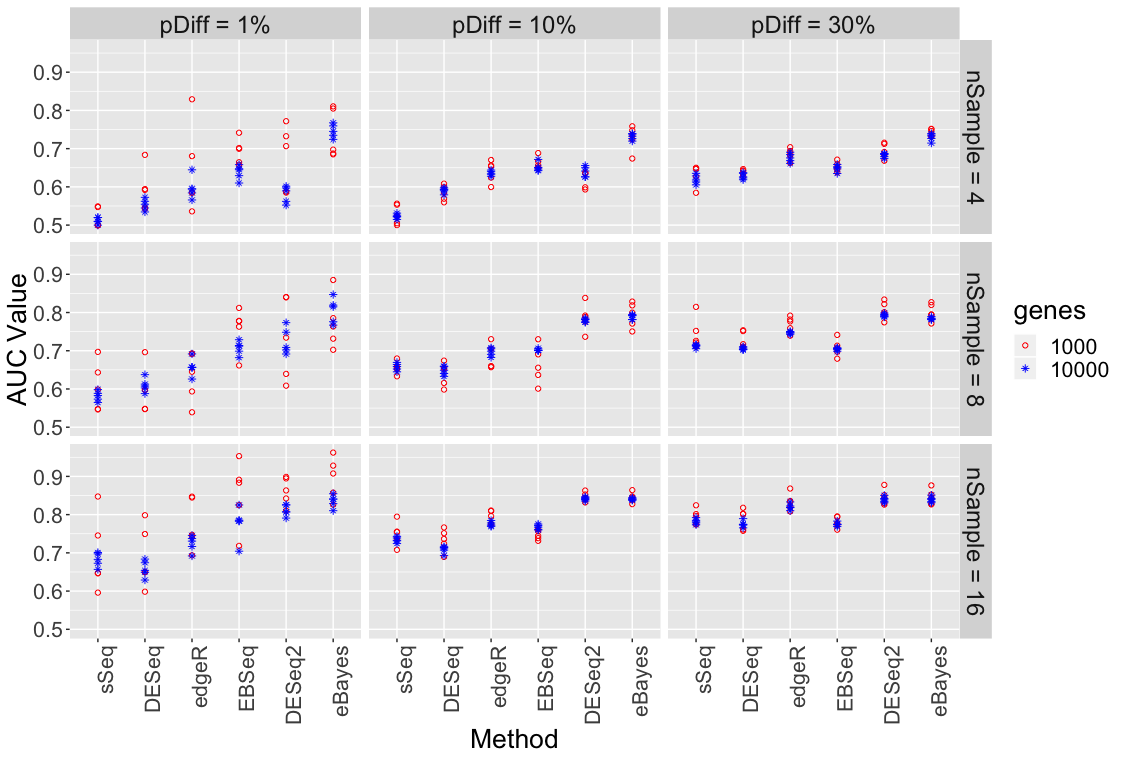
\includegraphics[height=10cm,width=15cm]{auc_plot}
\caption{AUC Plot of Simulated Datasets across Six Methods, Facetted by proportion of DE (pDiff) and number of samples (nSample), Grouped by total number of Genes (nGenes)}
\label{auc}
\end{figure}


We also evaluated the different methods with another performance metric: area under the curve (AUC) of ROC curves. Figure \ref{auc} provides the area under the ROC curve (AUC) across the 5 simulations for each of the scenario defined in \ref{tab:Scenario}. We facetted the plots by number of samples (nSample) and differential gene expression proportion (pDiff), grouped by different level of total number of genes. Similar to the single ROC curve, the eBayes method appears to outperform the other methods in terms of AUC, when number of samples and true DE proportion are small. With four or eight replcates per variety, there does not appear to be much of a difference between {\tt eBayes} and {\tt DESeq2}, but as the number of replicates decreases, the {\tt eBayes} approach appears to improve relative to {\tt DESeq2}.



We noticed that the difference among methods shrank as proportion of DE genes (pDiff) increases. The number of genes (nGenes) doesn't affect the methods performance in terms of AUC values. All methods perform better when the number of samples increases.


\section{Discussion}

{\tt eBayes} method is based on obtaining estimate for hyperparameters followed by MCMC to estimate gene-specific parameters. The empirical Bayes posteriors can be used to estimate posterior probabilities of DE . Through a simulation study, we demonstrated that this method outperformed alternative methods. 

Number of samples (nSamples) shows an impact on methods' performance in terms of AUC values. More samples (nSamples) would improve all methods' performance given the same proportion of DE genes (pDiff). DE analysis methods work better on count data with more replicates per condition and higher true DE genes proportion. This is not surprising considering that the focus of most methods is to model the variability in gene expression measurements and therefore increasing the number of replicates strengthen the estimate. 

The true DE genes proportion (pDiff) affects the outperformance of {\tt eBayes}. When pDiff is smaller, {\tt eBayes} performs much better than other methods in terms of AUC values, which means eBayes method has more advantages handling smaller true DE proportion scenario.

{\tt eBayes} method might be improved by refining the hierarchical model for the gene-specific parameter distribution and the hyperparameters estimation. There are other methods to explore, such as fully Bayesian methods. 



\section{Appendix}

\begin{figure}[h!tb] 
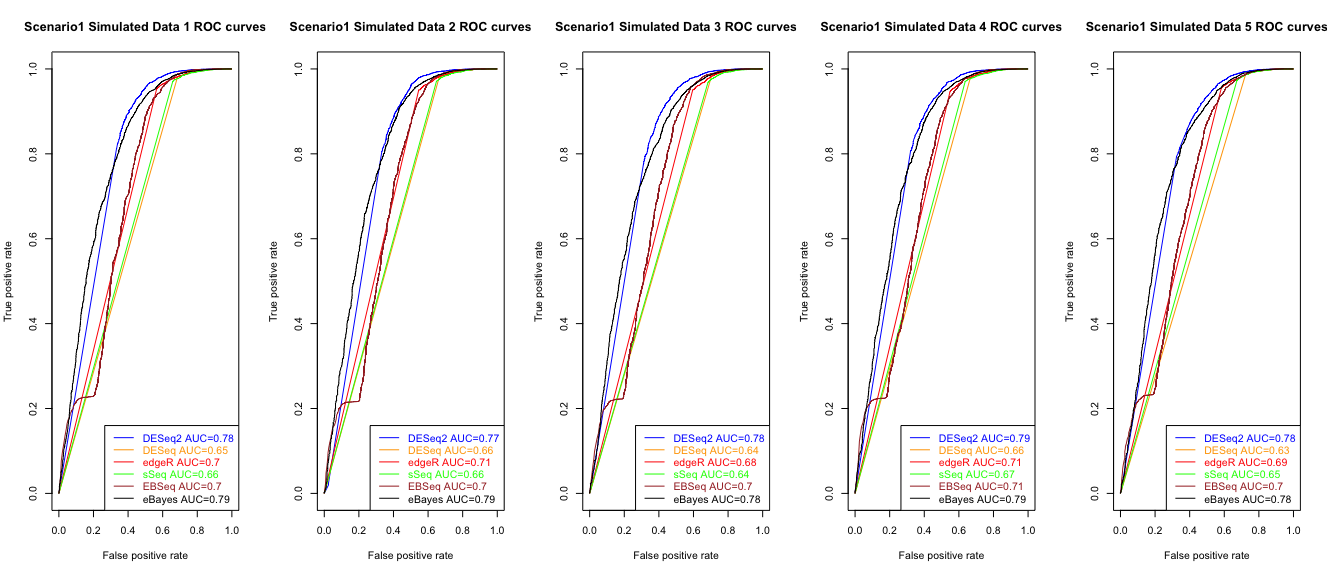
\includegraphics[height=6cm,width=15cm]{sc1_roc}
\caption{ROC curves of Simulated Datasets with $nGenes=10000, nSamples=8, pDiff=10\%$}
\label{sc1_roc}
\end{figure}



\begin{figure}[h!tb] 
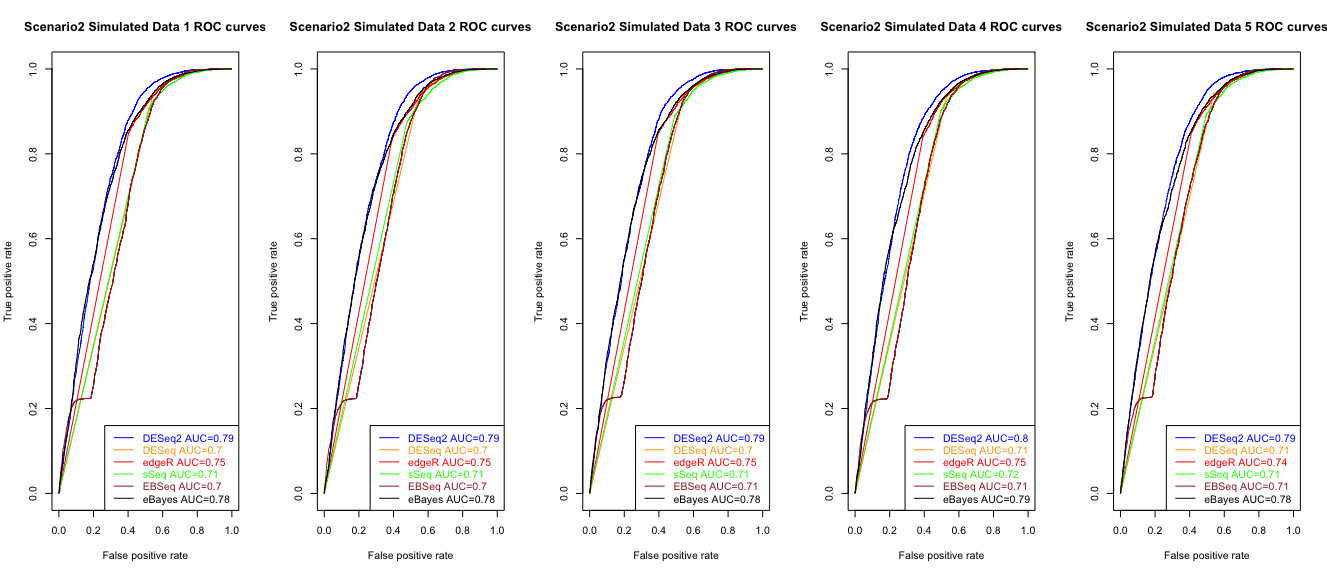
\includegraphics[height=6cm,width=15cm]{sc2_roc}
\caption{ROC curves of Simulated Datasets with $nGenes=10000, nSamples=8, pDiff=30\%$}
\label{sc2_roc}
\end{figure}

\begin{figure}[h!tb] 
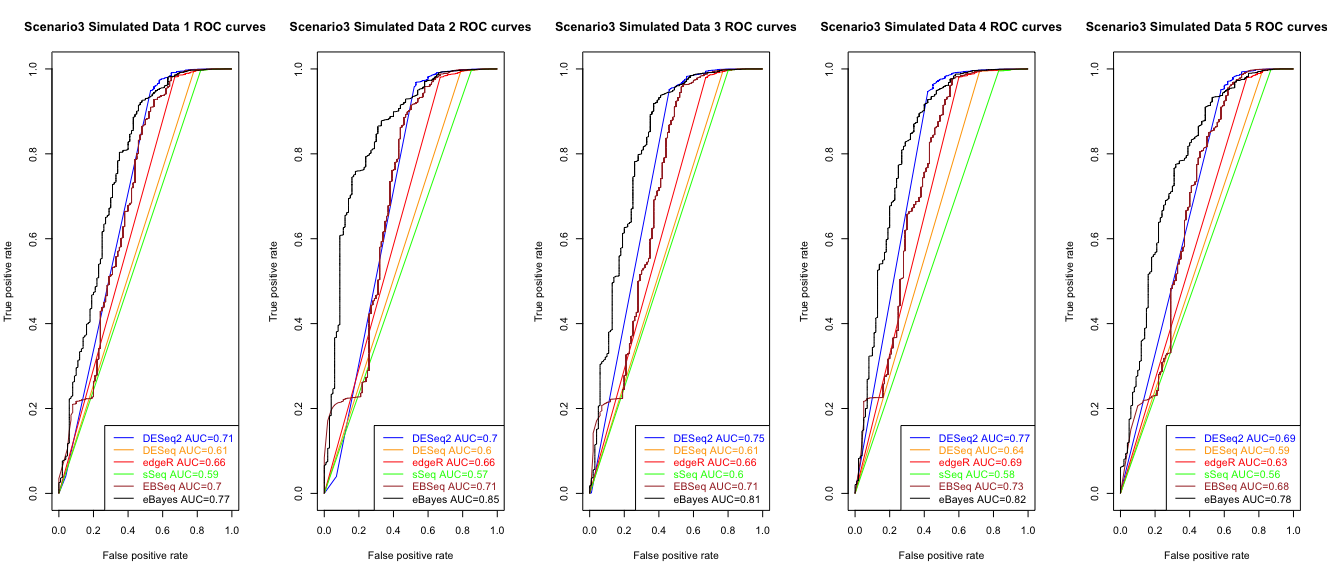
\includegraphics[height=6cm,width=15cm]{sc3_roc}
\caption{ROC curves of Simulated Datasets with $nGenes=10000, nSamples=8, pDiff=1\%$}
\label{sc3_roc}
\end{figure}


\begin{figure}[h!tb] 
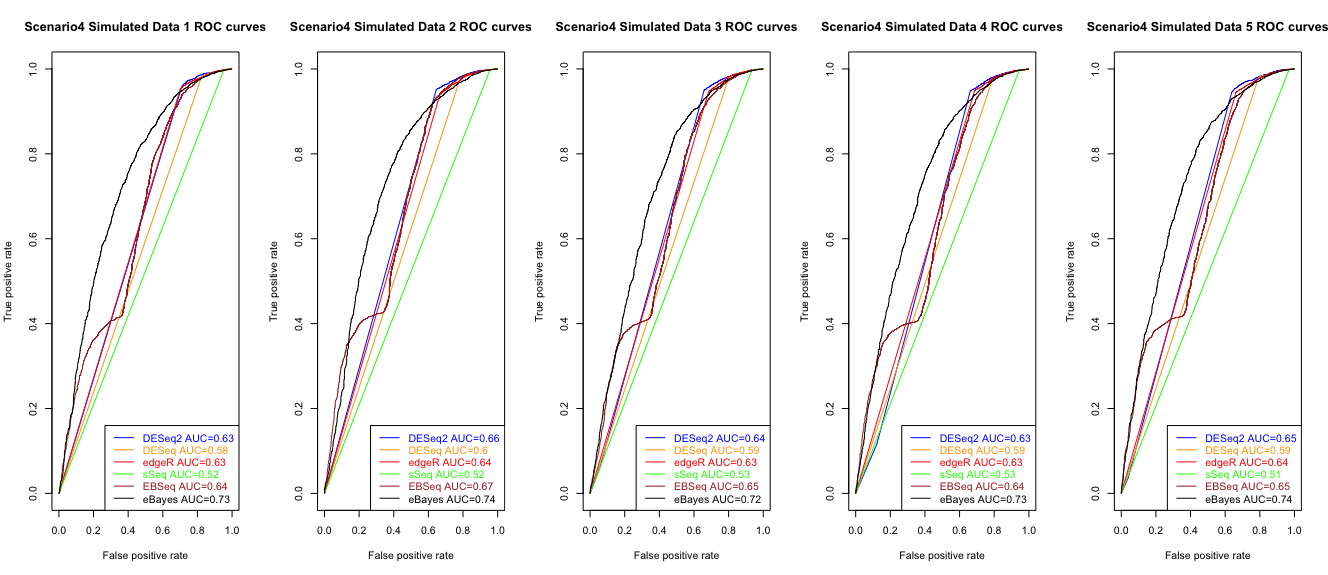
\includegraphics[height=6cm,width=15cm]{sc4_roc}
\caption{ROC curves of Simulated Datasets with $nGenes=10000, nSamples=4, pDiff=10\%$}
\label{sc4_roc}
\end{figure}


\begin{figure}[h!tb] 
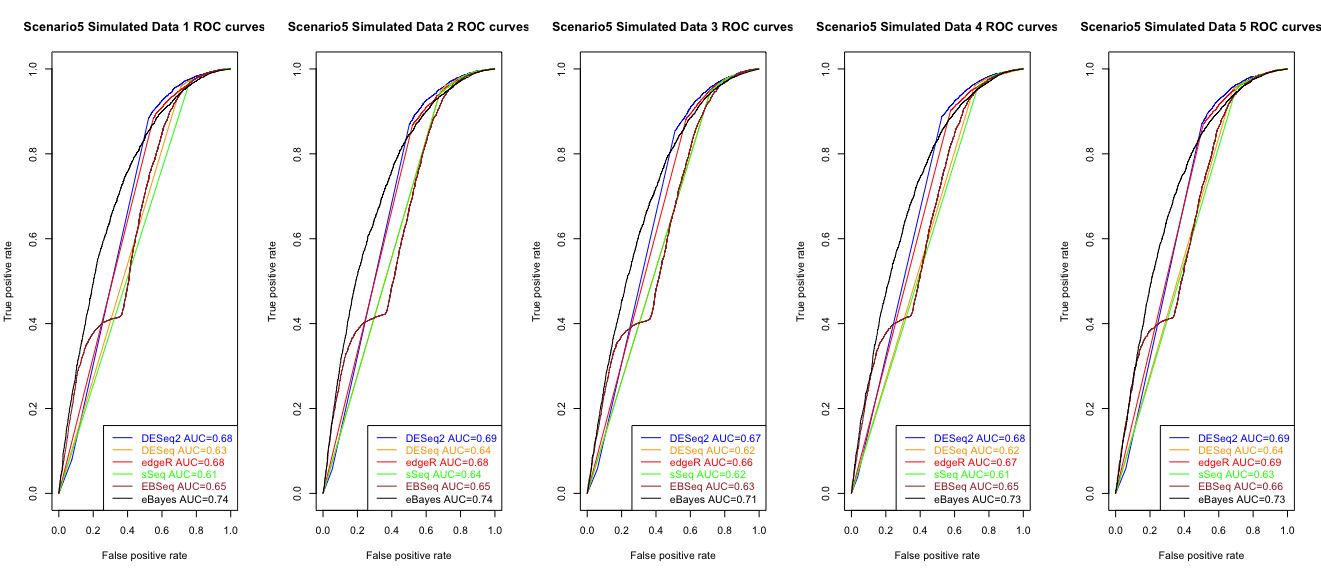
\includegraphics[height=6cm,width=15cm]{sc5_roc}
\caption{ROC curves of Simulated Datasets with $nGenes=10000, nSamples=4, pDiff=30\%$}
\label{sc5_roc}
\end{figure}


\begin{figure}[h!tb] 
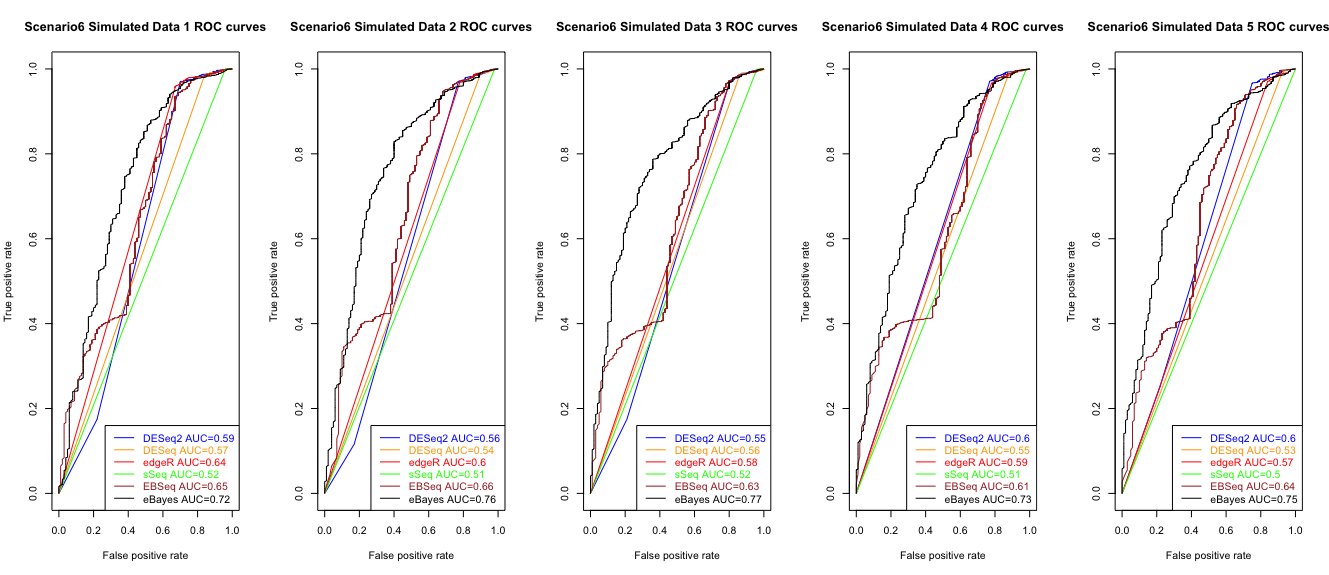
\includegraphics[height=6cm,width=15cm]{sc6_roc}
\caption{ROC curves of Simulated Datasets with $nGenes=10000, nSamples=4, pDiff=1\%$}
\label{sc6_roc}
\end{figure}

\begin{figure}[h!tb] 
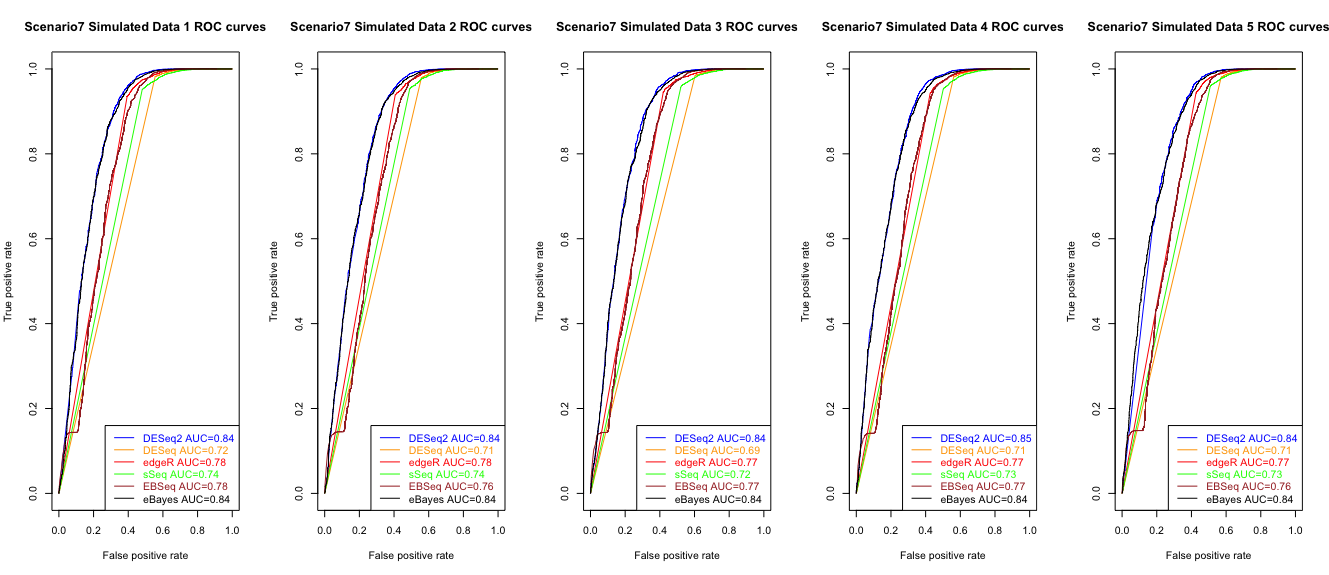
\includegraphics[height=6cm,width=15cm]{sc7_roc}
\caption{ROC curves of Simulated Datasets with $nGenes=10000, nSamples=16, pDiff=10\%$}
\label{sc7_roc}
\end{figure}

\begin{figure}[h!tb] 
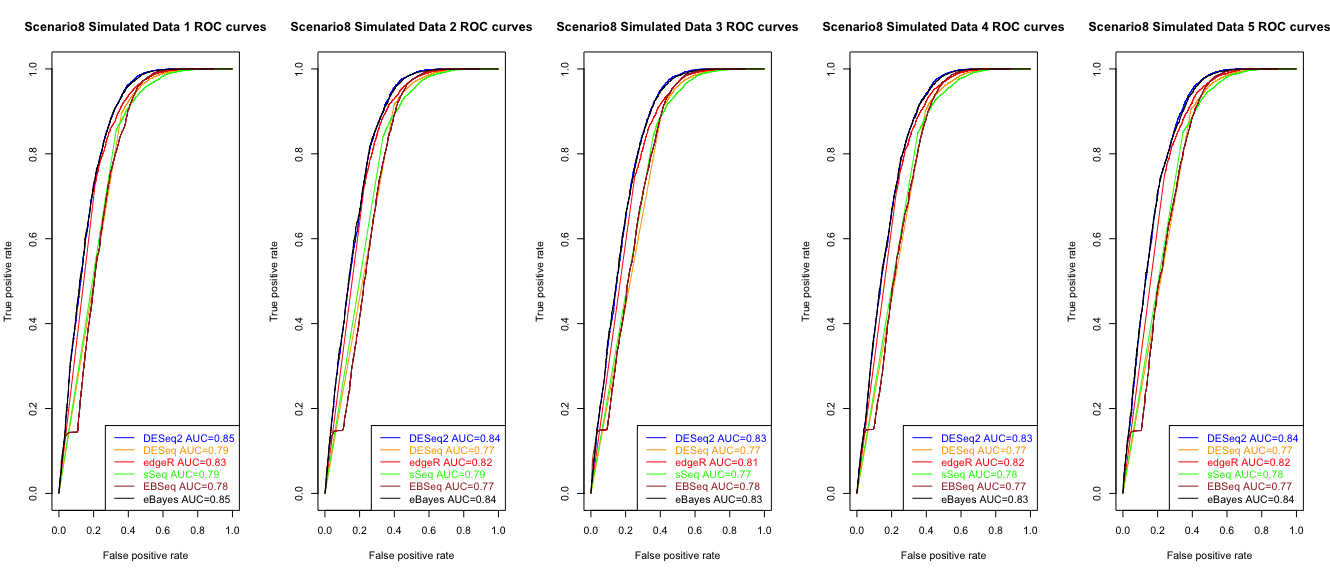
\includegraphics[height=6cm,width=15cm]{sc8_roc}
\caption{ROC curves of Simulated Datasets with $nGenes=10000, nSamples=16, pDiff=30\%$}
\label{sc8_roc}
\end{figure}

\begin{figure}[h!tb] 
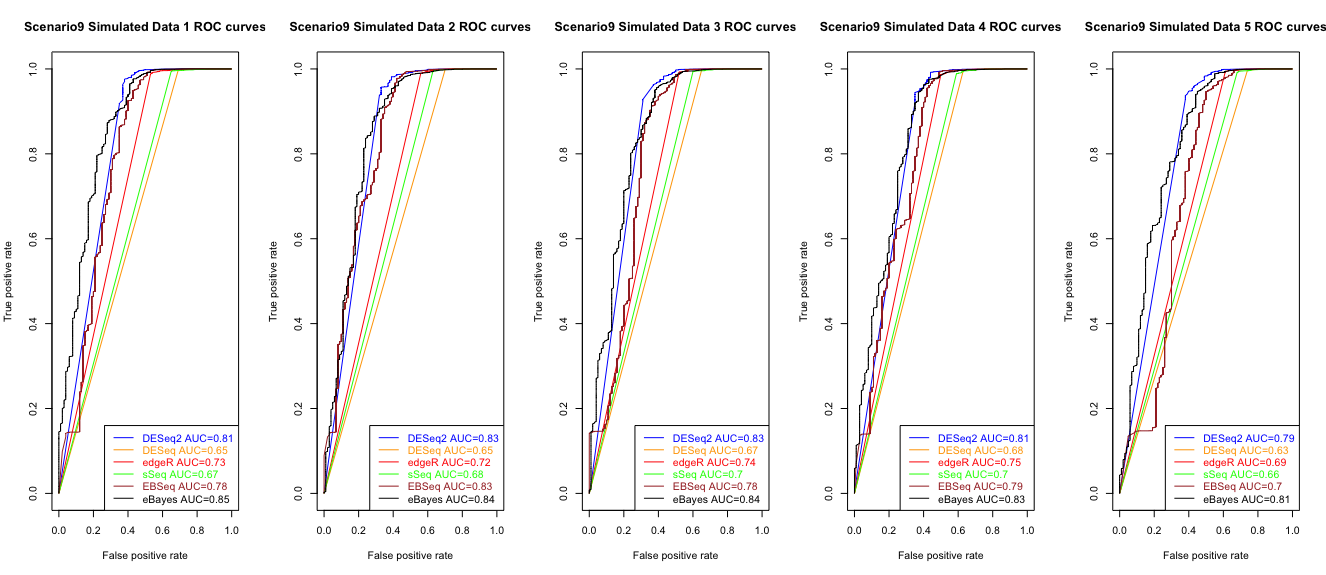
\includegraphics[height=6cm,width=15cm]{sc9_roc}
\caption{ROC curves of Simulated Datasets with $nGenes=10000, nSamples=16, pDiff=1\%$}
\label{sc9_roc}
\end{figure}


\begin{figure}[h!tb] 
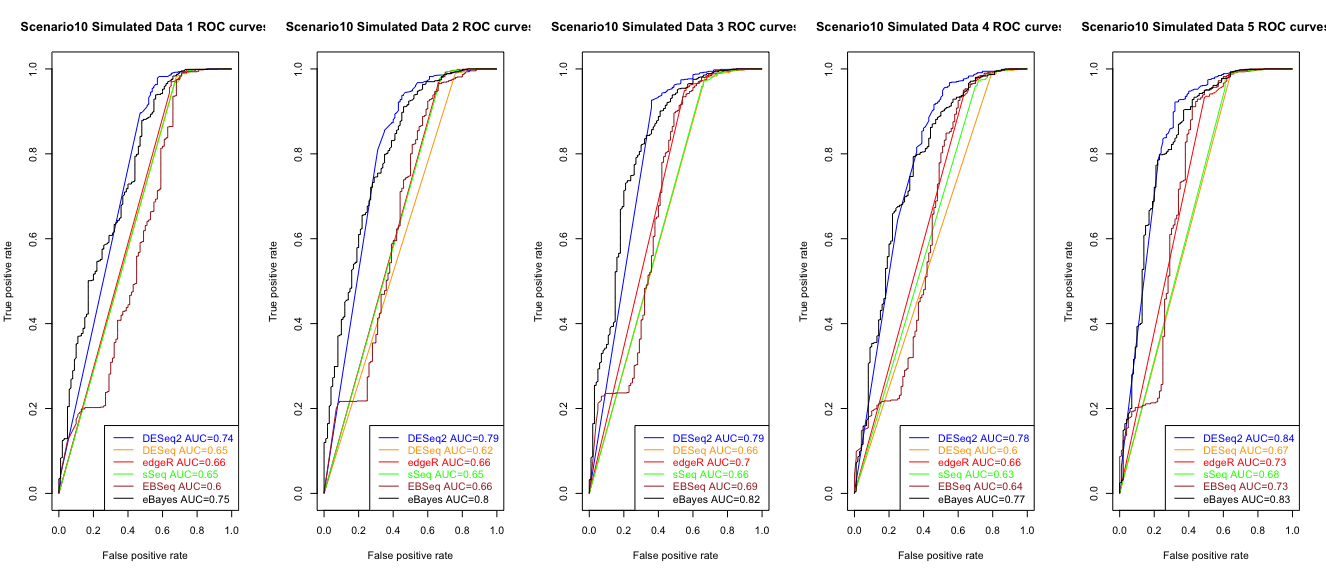
\includegraphics[height=6cm,width=15cm]{sc10_roc}
\caption{ROC curves of Simulated Datasets with $nGenes=1000, nSamples=8, pDiff=10\%$}
\label{sc10_roc}
\end{figure}




\begin{figure}[h!tb] 
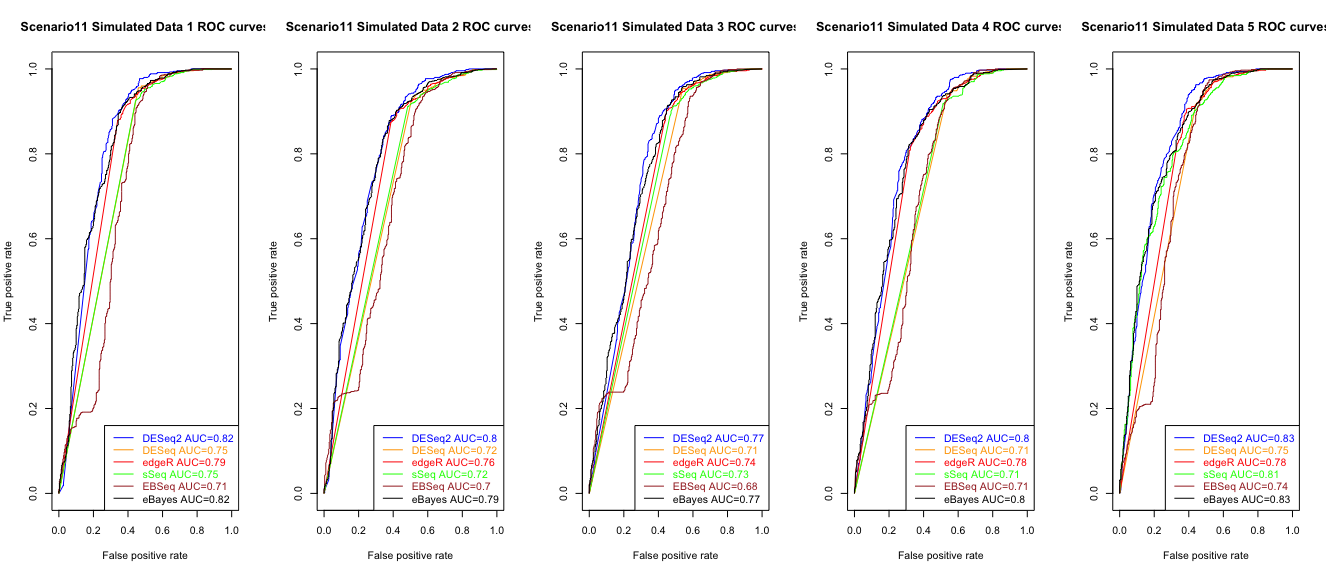
\includegraphics[height=6cm,width=15cm]{sc11_roc}
\caption{ROC curves of Simulated Datasets with $nGenes=1000, nSamples=8, pDiff=30\%$}
\label{sc11_roc}
\end{figure}

\begin{figure}[h!tb] 
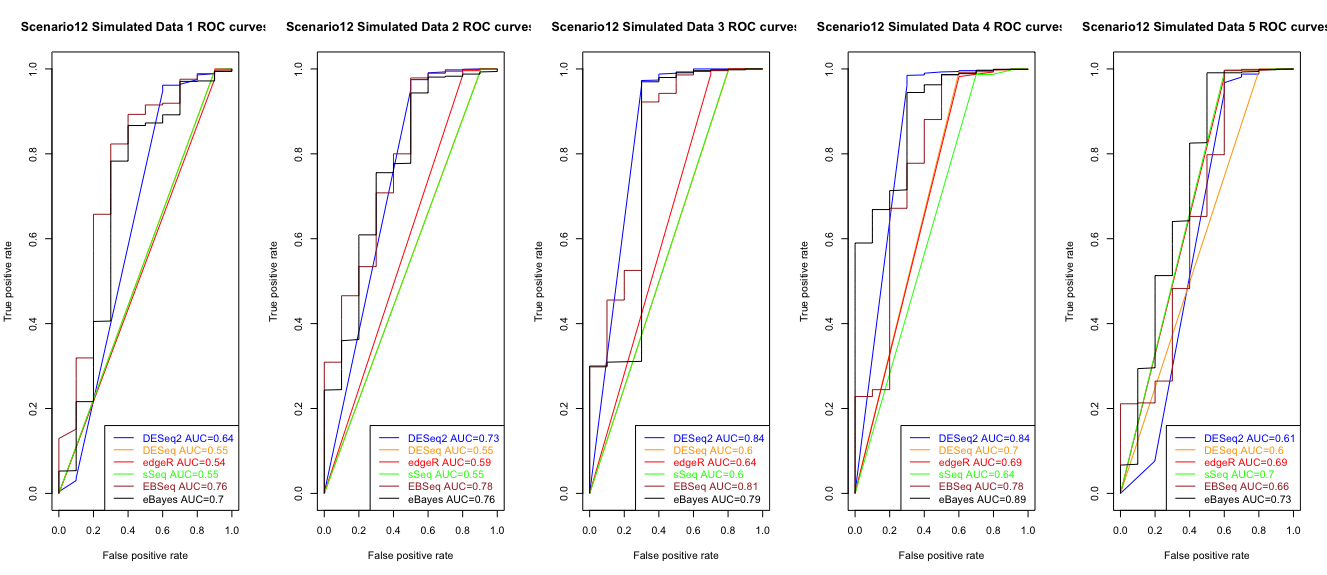
\includegraphics[height=6cm,width=15cm]{sc12_roc}
\caption{ROC curves of Simulated Datasets with $nGenes=1000, nSamples=8, pDiff=1\%$}
\label{sc12_roc}
\end{figure}


\begin{figure}[h!tb] 
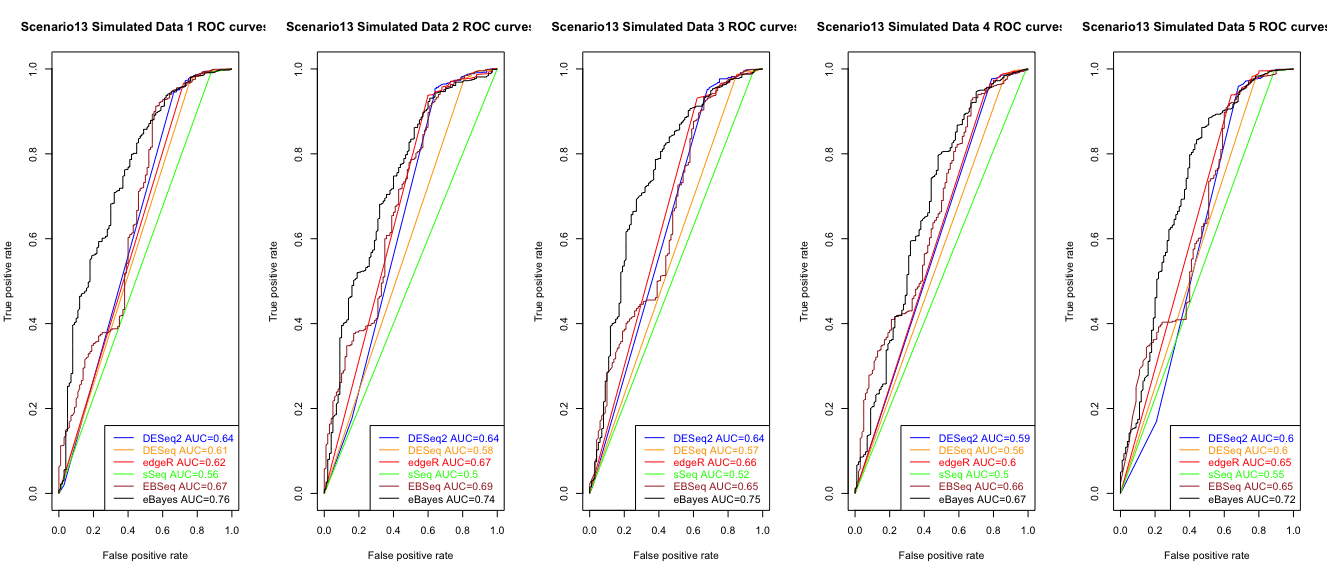
\includegraphics[height=6cm,width=15cm]{sc13_roc}
\caption{ROC curves of Simulated Datasets with $nGenes=1000, nSamples=4, pDiff=10\%$}
\label{sc13_roc}
\end{figure}


\begin{figure}[h!tb] 
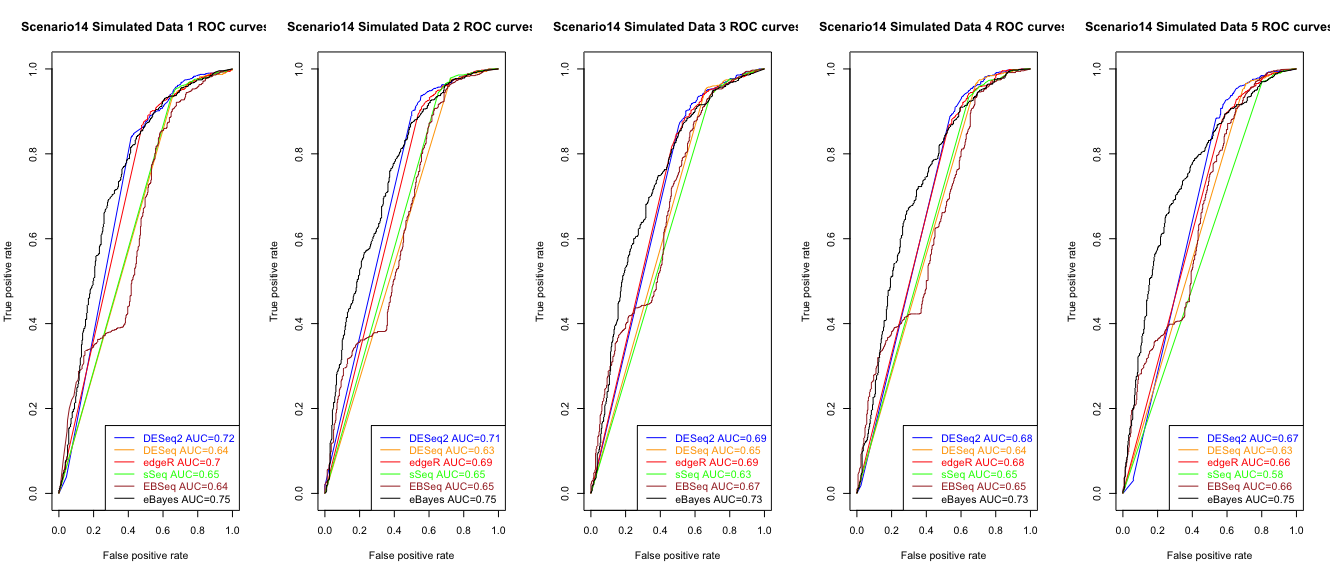
\includegraphics[height=6cm,width=15cm]{sc14_roc}
\caption{ROC curves of Simulated Datasets with $nGenes=1000, nSamples=4, pDiff=30\%$}
\label{sc14_roc}
\end{figure}


\begin{figure}[h!tb] 
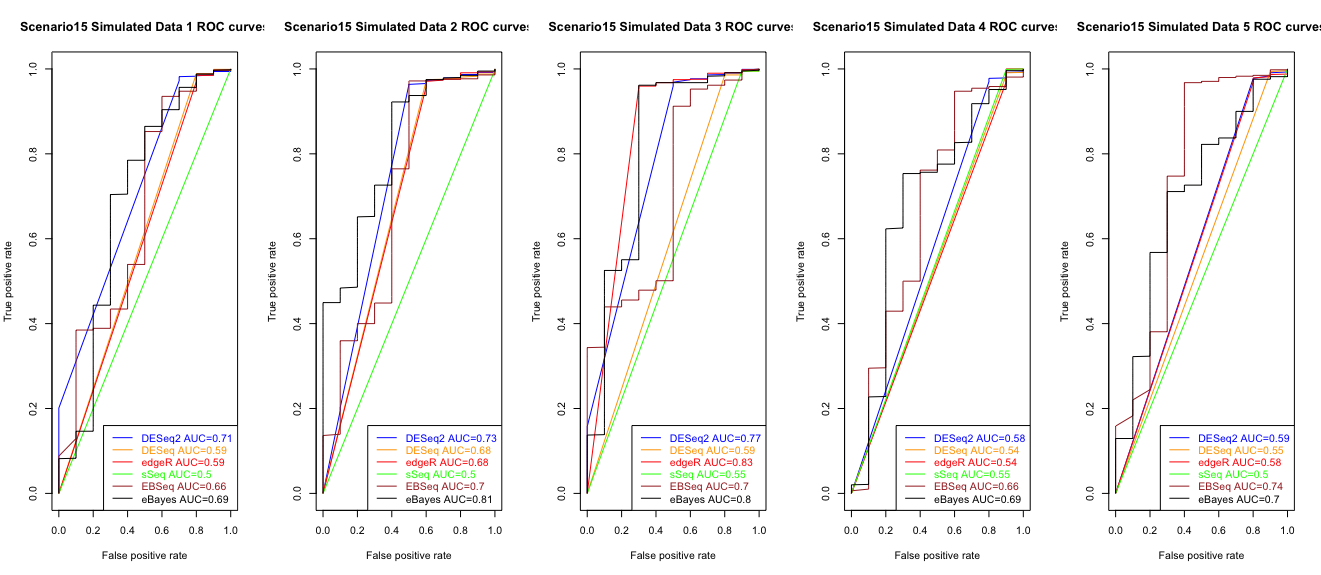
\includegraphics[height=6cm,width=15cm]{sc15_roc}
\caption{ROC curves of Simulated Datasets with $nGenes=1000, nSamples=4, pDiff=1\%$}
\label{sc15_roc}
\end{figure}

\begin{figure}[h!tb] 
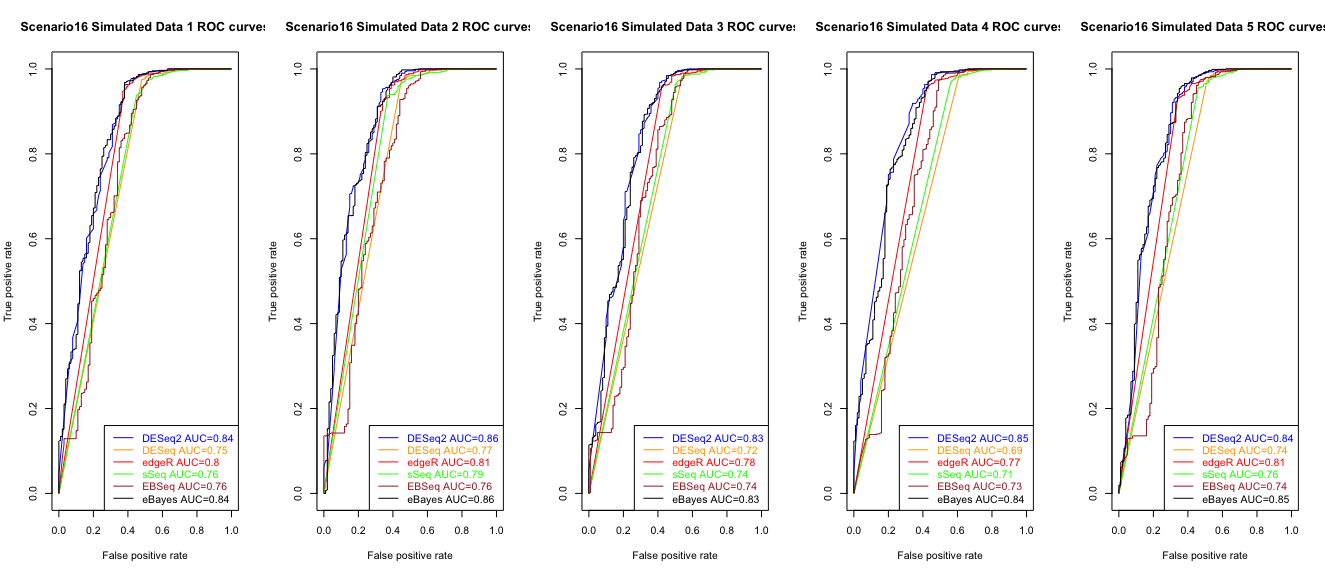
\includegraphics[height=6cm,width=15cm]{sc16_roc}
\caption{ROC curves of Simulated Datasets with $nGenes=1000, nSamples=16, pDiff=10\%$}
\label{sc16_roc}
\end{figure}

\begin{figure}[h!tb] 
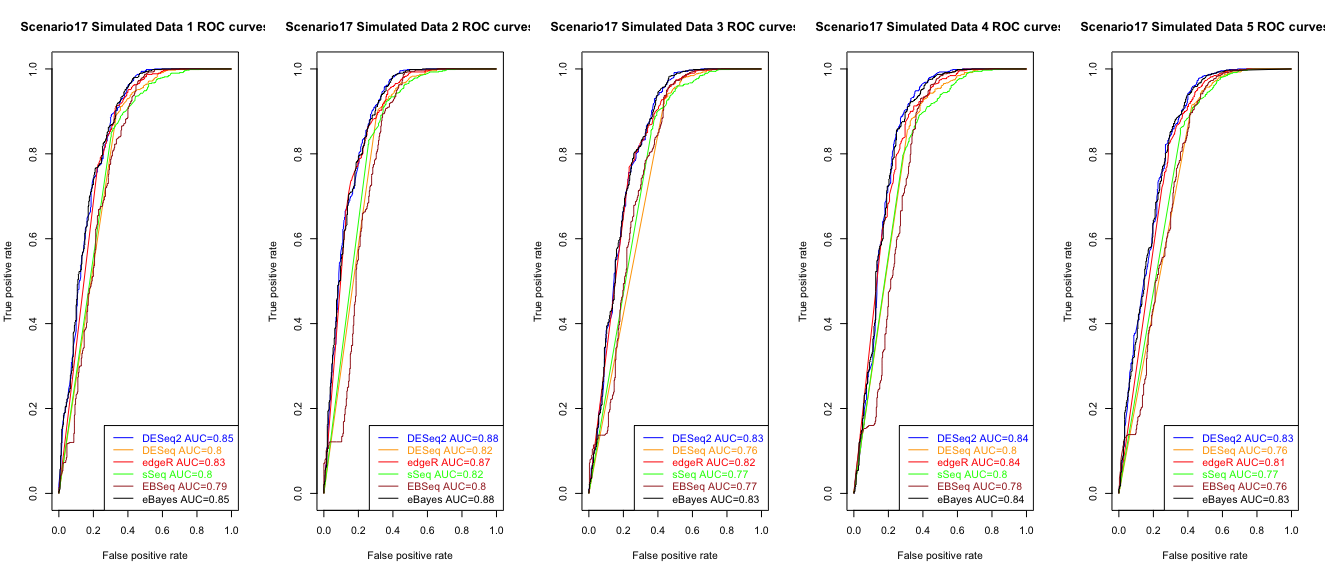
\includegraphics[height=6cm,width=15cm]{sc17_roc}
\caption{ROC curves of Simulated Datasets with $nGenes=1000, nSamples=16, pDiff=30\%$}
\label{sc17_roc}
\end{figure}

\begin{figure}[h!tb] 
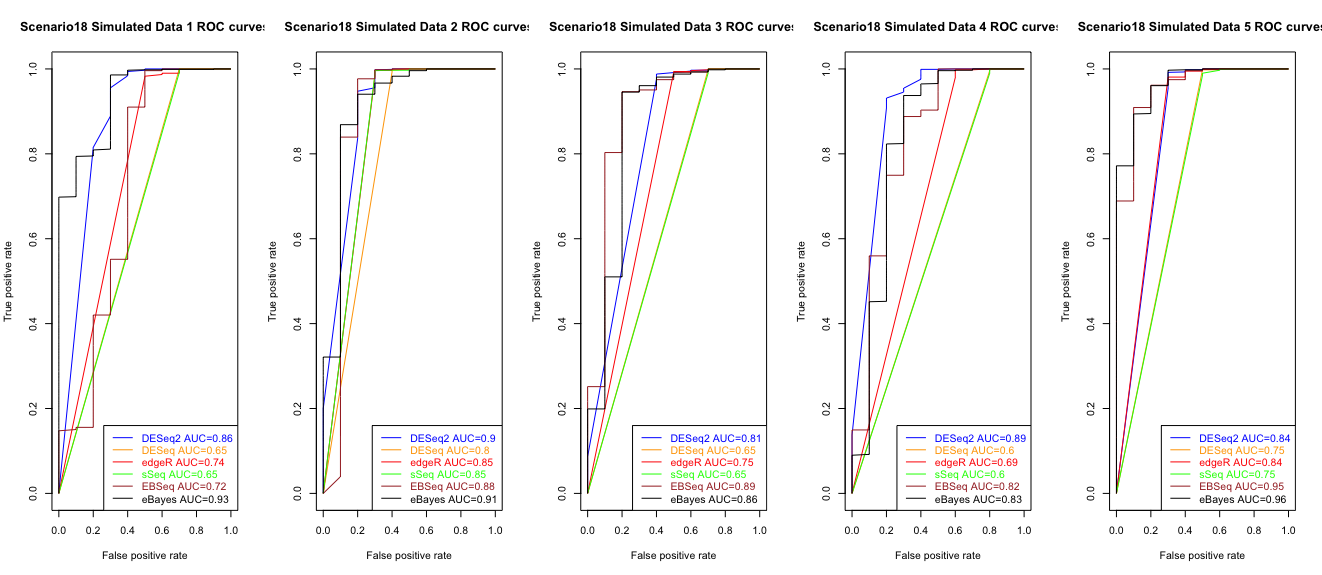
\includegraphics[height=6cm,width=15cm]{sc18_roc}
\caption{ROC curves of Simulated Datasets with $nGenes=1000, nSamples=16, pDiff=1\%$}
\label{sc18_roc}
\end{figure}
